\Tsec{Билет №4.2}

\begin{leftrules}
Генерация второй гармоники в случае слабого преобразования; роль расстройки. Факторы, ограничивающие эффективность преобразования, связь с расстройкой. Роль длины среды. 
\\ \phantom{42} \hfill \textit{лекция 2, слайды 13-23, лекция 3}
\end{leftrules}


\begin{to_def}
    \textit{''Заданное поле накачки''} - случай, когда, хоть и расстройка ненулевая (вообще говоря, любая), но амплитуда второй гармоники мала и не особо ослабляет амплитуду накачки (аппроксимируемо постоянной).
\end{to_def}

\textit{При заданном поле накачки} решение ур-я для медленных амплитуд:
\begin{equation*}
    G=\frac{2\pi \omega}{cn}\chi_{2}, \hspace{5 mm} \left\{\begin{aligned}
        A_{2\omega}(z)/A_{\omega}&=iGA_{\omega}z \sinc(\Delta k z/2) e^{-i\Delta k z/2} \\
        A_{\omega}(z)&=\const
    \end{aligned}\right.
\end{equation*}
где наблюдается периодические изменение интенсивности второй гармоники по длине среды (из-за sink) между нулем и тем большим значением, чем меньше расстройка. При фиксированной длине среды интереснее подобрать меньшую расстройку. Половина интенсивности теряется уже при $\Delta k L \simeq 2.8$ ($L$ - длина среды).


\textit{Среди причин ограничения эффективности:}
\begin{enumerate*}
    \item Пространственная неоднорожность пучка:
    пучок накачки в лучем случае гауссовый, так что на его крыльях $A_{\omega}(0)$ падает, из-за чего падает и $th$, что влечет на выходе наложении $\simeq 100\%$ эфф-ти от центра пучка и плохой эфф-ти от крыльев, что понижает общую эфф-ть; 
    \item  Временная неоднородность пучка: 
    проблема аналогична п. 1; 
    \item Нарушение частотного синхронизма: 
    нулевая расстройка для частоты накачки влечет ненулевую расстройку для спектральных крыльев накачки, что понижает эфф-ть:
    \begin{equation*}
        \Delta k \simeq [k_{2\omega}(2\omega_{0})+2\frac{dk_{2\omega}}{d\omega}(\omega-\omega_{0})]+[2k_{\omega}(\omega_{0})+2\frac{dk_{\omega}}{d\omega}(\omega-\omega_{0})] = 2(\omega-\omega_{0}) \big( v_{gh}^{-1}(2\omega) - v_{gr}^{-1}(\omega) \big)
    \end{equation*}, так что решение - ограничение спектра накачки: $\Delta \omega < \frac{2,8}{\tau (2\omega) - \tau (\omega)}$, где $\tau$ - групповое время запаздывания $\implies$ время импульса лазера $\tau > \tau(2\omega)-\tau(\omega)$;  
    \item Нарушение углового синхронизма: 
    например, в одноосном кристалле дифракционное уширение пучка влечет уширение пучка второй гармоники, которая является в одноосном кристалле необыкновенной волной, а значит ее пок-тель преломл. зависит от угла, и это все приводит к нарушению фазового синхронизма: $\Delta k = \frac{2\omega n_{2\omega}}{c}\alpha (\theta - \theta_{0})$, где $\alpha = \frac{1}{n}n'_{\theta}$ - угол сноса, в стандартных лазерах на стандартных кристаллах равный единицам градусов (не мало). Короче, условие на ширину пучка: $D \leq 2L \alpha$ ($l$ - длина среды).
\end{enumerate*}


\textit{Решение проблем ограничения эфф-ти:} \textbf{1)} 90-тиградусный синхронизм: угол сноса в таком случае нулевой; \textbf{2)} периодически поляризованный кристалл: кристалл состоит чередующихся доменов с двумя разными направлениями нелинейной полярной оси, что компенсирует расстройку фазового синхронизма; \textbf{3)} резонатор: накачку вносят в резонатор Фабри-Перо, который на порядка 2-3 увеличивает ее, как и вторую гармонику.


\begin{figure}[ht]
    \centering
    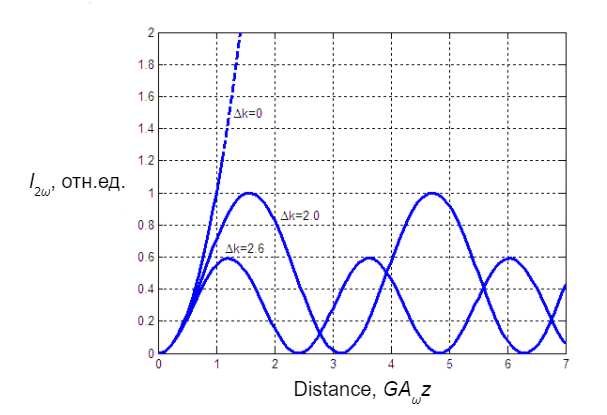
\includegraphics[width=0.5\textwidth]{figures/4_2.png}
    \caption{Постоянная волна накачки}
    %\label{fig:}
\end{figure}
